\section{Hardware Implementation\label{sec:Hardware-Implementation}}


\subsection{Methodology}

Commonality between modules, same life-support system.


\subsection{CAD Design}

Schematic capture and PCB layout using EagleCAD.


\subsection{Commonalities}

All 4 modules are implemented on custom printed circuit boards (PCBs) with an \emph{AT90CAN128} micro-controller from Atmel. Programming and debugging software on the microcontroller was done through a standard IEEE 1149.1 JTAG interface. The module is linked to the other system modules with a CAN bus. All inter-module communication is done over the CAN bus.

\subsubsection{Microcontroller}


\subsubsection{CAN Transceiver}


\subsubsection{Linear Regulator}


\subsubsection{Supervisor}


\subsubsection{Wiring Harness}


\subsection{Engine and Transmission Module}

<Picture of board>

Overview of physical implementation.


\subsubsection{High Current Solenoid Driver}


\subsubsection{Input Buffers}


\subsubsection{Traction Control Analogue Output}

The ECU allows a 0-5v analogue input to modify the allowable traction slip ratio from 0-100\% for the traction control.

The Engine module uses a simple SPI interfaced DAC from Texas Instruments, the TLV5623, to output the 0-5v analogue signal to the ECU.

The output voltage from the DAC is given by

\begin{equation}
V_{out}=2\cdot{V_{ref}}\,\frac{Code}{2^{n}}\,[V]
\end{equation}

where $V_{ref}$ is the reference voltage input to the chip, $n=8\,(bits)$, and $Code$ is the digital input value ranging from $0$ to $2^{n-1}$. Since we want to output $5\,[V]$ at fullscale input, \begin{equation} 2\cdot{V_{ref}}\,\frac{2^{7}}{2^{8}}=V_{ref}=5\,[V]\end{equation}.

The DC input resistance $R_{in}$ on the traction cut input pin on the ECU was measured using a series resistor with the input terminal to be $R_{in}\approx155k\Omega$. The output current of the DAC therefore will be at most $I_{out}=\frac{5v}{155k}\approx32.26\mu A$.

\subsection{Braking Module}

\begin{figure}[h]
\centering
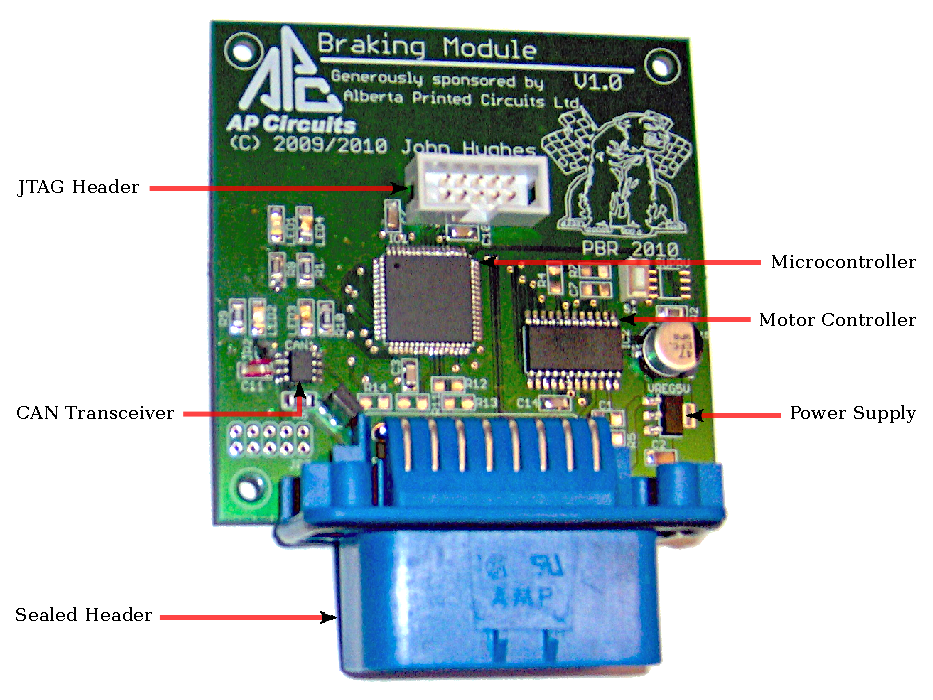
\includegraphics[scale=1]{implementation/figures/braking_pcb}
\caption{Populated Braking module PCB.}
\label{fig:braking_pcb}
\end{figure}

The braking module implementation was the simplest of the 4 modules in terms of electrical design. Only one special component on the board was required, a stepper motor controller/driver, and the interface to the microcontroller only required a handful of i/o lines. Additionally, a pressure transducer was also specified to facilitate measuring the hydraulic pressure in the brake lines. The components chosen for the braking module are listed in Table \ref{table:braking_module_components}.

Figure \ref{fig:braking_pcb} shows a photograph of the completed braking module circuit board, with all components soldered on. The simplicity of the electrical design is reflected in the fact that no additional corrections (other than for the CAN transceiver) were required for the module to be 100\% operational.

\begin{table}
  \caption{Braking module components.\label{table:braking_module_components}}
  \centering
  \begin{tabular}{|c|c|c|}
    \hline 
    Part & Manufacturer & Part Number\tabularnewline 
    \hline \hline
    Stepper Motor Controller/Driver & Allegro Microsystems & A3967 \tabularnewline
    \hline
  \end{tabular}
\end{table}

\subsubsection{Stepper Motor Driver}

In order to meet the design goal of having the implementation be flexible in terms of which stepper motor would be used in the system, a current-sensing stepper motor controller/driver component was used in the circuit design. The current sense capability allows us to fix the input voltage in the circuit design, and afterwards adjust the current drive by changing resistor values in the current-sense feedback loop. 

The A3967 "Microstepping Driver with Translator" was chosen to drive the stepper motor for several reasons. The A3967 integrates a microstepping controller with dual H-Bridge output stages into one package. This simplified the potential circuit design. The H-Bridge output transistors can supply up to $\pm\unit{750}{\milli\ampere}$ of current at up to \unit{30}{\volt} \cite{A3967}. This flexibility was desirable.

\paragraph{Current Control}
\nomenclature{$R_{sense}$}{Value of the current sense resistors in the Braking Module's stepper motor circuit.}
\nomenclature{$I_{TRIP}max$}{Maximum current allowed to flow into the Braking Module's stepper motor before the PWM circuit shuts the output stage off.}

The current control feature of the A3967 works by sensing the current through a sense resistor, $R_{sense}$, and varies the duty cycle of a fixed off-time PWM circuit, which controls the output from the H-Bridge stages.

The value of the sense resistor was determined by an equation recommended in the datasheet:
\begin{equation}
R_{sense}=\frac{0.5}{I_{TRIP}max}
\end{equation}
where $I_{TRIP}max$ is the maximum current allowed to flow into the motor before the PWM circuit shuts the output stage off.

\subsubsection{Analogue-to-Digital Converter}


\subsubsection{End-of-Travel Microswitches}

\subsection{Telemetry Module}


\subsubsection{Wireless Modem}

To meet the range and data throughput requirements for the telemetry system, an XBee Pro wireles modem was used. The XBee requires 3.3v I/O levels and power supply, and so a second linear voltage regulator was used in the design, the LT1521 from Linear Technology. Since the AT90CAN129 has only 2 built-in UARTS that were used for the RS232 interfaces to the ECU and DAQ, an third external UART was added to the design. The MAX3100 is a SPI-interfaced UART with an 8 word deep FIFO buffer. It is interfaced to the AT90CAN128's SPI pins and has an active-low IRQ line connected to external interrupt line EXT7 on the microcontroller. 

The wireless transmitter is an XBee Pro Modem from Digi International. The modem is in a package designed for mounting on a printed circuit board, and is attached to the telemetry module directly. This modems requires a 3.3V power supply. and consumes at most 215mA of current during transmit. Since the common module hardware only provides power for 5V devices, the telemetry module has a second LDO regulator providing 3.3V. A separate antenna port is connected to the modem and mounted in the side of the module enclosure.



\subsubsection{External SPI USART}


\subsubsection{Two-Channel ECU and DAC USART}

\subsection{Driver Interface Module}


\subsubsection{Steering Wheel Unit}


\subsubsection{LCD Module Bias Circuit}

The LCD screen requires a large bias voltage of +22V.

A Linear Technology LT1615 step-up DC/DC converter was chosen as the centre of a boost converter circuit for the LCD.


\paragraph{Inductor Selection}

\begin{equation}
L=\frac{V_{out}-V_{in(min)}+V_{D}}{I_{limit}}\cdot t_{off}\label{IndSel}
\end{equation}


Using (\ref{IndSel}) with $V_{D}=0.4V$, $I_{limit}=350mA$, $t_{off}=400ns$, $V_{out}=+22V$, and $V_{in(min)}=11.5V$ gives $L\approx12.45\mu{H}$. The datasheet however suggests a value slightly smaller than calculated should be suitable with only slight decrease in maximum output current. Since the LCD requires very little current, we used an inductor value of $10\mu H$.


\paragraph{Output Voltage}

To obtain a $V_{bias}$ of $+22V$, two resistors in the bias circuit provide a voltage divided feedback path from the output to the FB pin on the LT1615. The eqation relating the output voltage with the resistor values is

\begin{equation}
R_{1}=R_{2}\cdot\left(\frac{V_{bias}}{1.23}-1\right)
\end{equation}

 $R_{1}$ was chosen to be $2M\Omega$ to limit current flowing from the output to ground, and a suitable $R_{1}$ of $118k\Omega$ was found.


\subsubsection{LCD Module Data Interface}

The LCD's 8-bit interface was suitable to be connected to the AT90's external memory interface. This way the LCD becomes a memory-mapped periferal to the AT90, and all the control signals (Read and Write strobes, etc.), are handled by the memory controller.

The AT90's external memory interface uses Port A pins 0-7 as a multiplexed data and address bus which must be demultiplexed in order to offer seperate address and data busses. In operation, the external memory interface first puts out the address on the combined bus, followed by the data. The ALE (Address Latch Enable) signal signifies the difference \cite{AT90CAN}.

In order to provide seperate address and data busses for the LCD controller, a fast octal D-Type latch from NXP was chosen to latch the address from the AT90. The width of the ALE pulse, $t_{LHLL}$, provided by the AT90, is specified in the datasheet as

\begin{equation}
t_{LHLL}=t_{CLCL}-15\, ns
\end{equation}

 where $t_{CLCL}$ is the clock period. With the clock running at $16\, MHz$, $t_{LHLL}=48\, ns$.

The 74LVC373A latch from NXP requires a minimum LE pulse width of $4.5\, ns$, so is suitable as a demultiplexing interface.

The external memory on the AT90CAN128 starts at address 0x1100h, and there are two possible registers to read/write to on the LCD controller. The LCD controller therefore has it's single address select pin connected to the LSB of the address lines output from the latch. Since only two addresses are required, the upper 8 address lines of the external memory interface were not used.

A logical combination of the lower byte address lines will be connected to the CS (Chip Select) line on the LCD controller. Since the external memory controller only outputs control signals when the requested memory operation is in external space, it is safe to ignore the upper byte address lines.

It was chosen to tie the 2nd bit of the address lines to CS, which provides the following table of operations when interacting with the LCD controller:

\begin{table}
\begin{centering}
\caption{Memory-mapped LCD Interface}

\par\end{centering}

\centering{}\begin{tabular}{|l|l|l|}
\hline 
Address  & Read Function  & Write Function\tabularnewline
\hline
\hline 
0x1102  & Status flag read  & Display data and parameter write\tabularnewline
\hline 
0x1103  & Display dada and cursor address read  & Command write\tabularnewline
\hline
\end{tabular}
\end{table}

\subsubsection{Input Knobs and Buttons}


\subsubsection{Paddle Shifters}